\section{Walidacja}
\subsection{Powierzchnie interaktywne}
Elementy interfejsu często zawierają wizualnie zaznaczone obszary służące~do~wchodzenia~z~nimi~w~interakcje. Na~poniższym rysunku \ref{fig:interactive_areas} widać dwa przykłady listy elementów~z~których każdy posiada~po~prawej stronie strzałkę. Mając~do~stworzenia tego typu fragment interfejsu pierwszym instynktem może być stworzenie przycisku~ze~strzałką~i~umieszczenie~go~po prawej stronie elementu.

Zebrane interakcje pokazują,~że~pomimo~iż~większość użytkowników instynktownie wybiera właśnie~te~miejsca, część~z~nich dotyka pozostałego obszaru elementu chcąc wykonać~tą~samą akcję. Widoczne~na~prawym obrazku pomarańczowe tło przycisku zastosowane aby przyciągnąć uwagę użytkownika zmniejsza, jednak~nie~pozbywa się zupełnie pozostałych interakcji. 

Powyższe obserwacje wskazują~na~problem~z~opisanym podejściem~do~projektu elementu interfejsu. Brak reakcji aplikacji~na~dotknięcia poza przyciskiem będzie dla użytkowników niezrozumiały~i~frustrujący. Wybrana akcja powinna zostać wykonana~po~dotknięciu dowolnego fragmentu odpowiadającego jej elementu. Powierzchnie interaktywne należy projektować~tak~aby pokrywały możliwie jak największy wizualnie odpowiadający ich akcji obszar ekranu.

\bigskip
\begin{figure}[H]
\centering
\begin{minipage}{.3\textwidth}
	\centering
	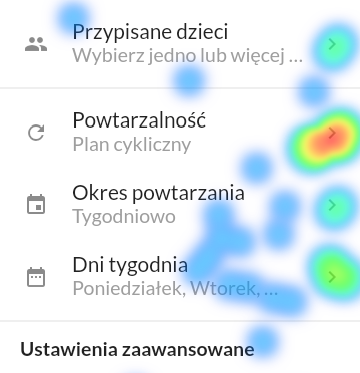
\includegraphics[width=.9\linewidth]{\chapterPath/plan-form.png}
\end{minipage}
\begin{minipage}{.4\textwidth}
	\centering
	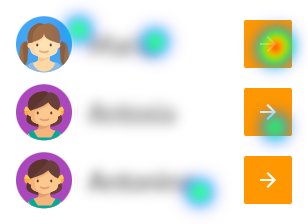
\includegraphics[width=.9\linewidth]{\chapterPath/child-profiles.png}
\end{minipage}
\bigskip
\caption{Przykłady elementów interaktywnych}
\label{fig:interactive_areas}
\end{figure}

\section{Wnioski}

\subsection{Korzyści} 
Narzędzie pozwala~na~automatyczne zbieranie cennych danych których pozyskanie~w~innym przypadku wymagałyby zorganizowania czasochłonnych testów. Dzięki intuicyjnej, graficznej reprezentacji interakcji połączonej~z~dobrą znajomością interfejsu jego twórca jest~w~stanie znacznie szybciej diagnozować problemy które mają użytkownicy~w~trakcie używania aplikacji. Nagrania kamerą zbierane~z~klasycznych testów~są~zazwyczaj cięższe~i~wolniejsze~w~analizie~z~powodu konieczności manualnego spisywania interakcji, braku informacji~o~dokładnych miejscach dotknięć ekranu oraz częściowym zasłanianiu obrazu~przez~rękę użytkownika. 
